\section{Theorie}
\label{sec:Theorie}
Laser steht für „Light Amplification by Stimulated Emission of Radiation“.
Er ist in der Forschung, speziell in der Spektroskopie, von großer Bedeutung, da er eine ideale Lichtquelle darstellt.
Das Licht eines idealen Lasers ist kohärent, monochromatisch, hat eine hohe Intensität und hält diese stabil.
Im Folgenden soll am Beispiel des Diodenlasers erläutert werden, wie eine solche Lichtquelle realisiert werden kann und 
wie er für die Spektroskopie der Hyperfeinstrukturaufspaltung von Rubidium genutzt werden kann.
\subsection{Funktionsweise eines Lasers}
Grundlegend besteht ein Laser aus drei Komponenten: einem aktiven Medium, einer Energiepumpe und einem Resonator.
Die Energiepumpe pumpt Energie in das System, indem Elektronen im aktiven Medium angeregt werden (z.B. über eine Blitzlampe, Gasentladung, einen weiteren Laser oder wie in diesem Fall über einen Strom von Ladungen).
Das Ziel der Energiepumpe ist es, eine Besetzungsinversion zu erzeugen. Das heißt, wie in Abbildung \ref{fig:inv} zu sehen, einen Zustand hoher Energie mit einer größeren Anzahl Elektronen zu besetzen 
als die energetisch darunter liegenden Zustände.
\begin{figure}[H]
    \centering
    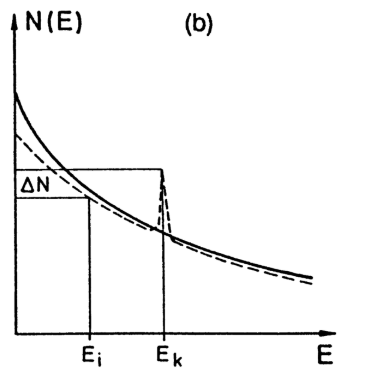
\includegraphics[scale=0.9]{pictures/Inv.png}
    \caption{Besetzungsverteilung eines aktiven Mediums \cite{Demtröder}.}
    \label{fig:inv}
\end{figure}
\noindent Die Elektronen regen sich durch verschiedene Emissionsprozesse unter der Aussendung eines Photons fester Energie ab.
Die Photonen werden dann im Resonator reflektiert und so wieder durch das aktive Medium hindurch geschickt,
wo sie durch stimulierte Emission weitere Photonen erzeugen. Dadurch wird der Laser zu einem selbst schwingenden Oszillator.
Diese Photonen sind dann kohärent. Ein Resonatorspiegel ist teildurchlässig, wodurch sich nach dem Hochfahren des Lasers ein Maximum einstellt. Danach wird durch den teildurchlässigen
Spiegel eine konstante Lichtintensität abgegeben. Je nach Resonatorkonfiguration speichert der Laser das Licht in festen Moden.
\subsection{Emission und Absorption im Aktiven Medium}
Zunächst sollten die wichtigsten Prozesse im aktiven Medium, anhand eines Zwei-Niveau-Systems diskutiert werden. 
Wie in Abbildung \ref{fig:Prozesse} zu sehen, gibt es drei zentrale Prozesse. Liegt ein System in einem angeregten Zustand vor, heißt das, dass ein Elektron auf dem Zustand höherer Energie vorliegt.
Es ist grundsätzlich energetisch günstiger für das Elektron in einem tieferen Zustand vorzuliegen. Tritt dieser Übergang ohne äußere Einflüsse auf, so wird ein Photon mit der entsprechenden Energiedifferenz zwischen den beiden Niveaus ausgesendet. Dies wird spontane Emission genannt.
Bewegt sich nun ein Photon mit genau der Energiedifferenz zweier Zustände eines Atoms auf dieses zu, kann es zu 2 Prozessen kommen.
Wenn das Elektron im niedrigeren Zustand vorliegt, kann das Photon absorbiert werden (Absorption) und 
das Elektron in den höheren Zustand übergehen. Liegt das Elektron im höheren Zustand vor, kann das Photon eine stimulierte Emission auslösen, bei der 
das Elektron in den niedrigeren Zustand übergeht und ein weiteres kohärentes Photon aussendet. Das Photon hat dann die gleiche Wellenlänge, Polarisation und Ausbreitungsrichtung wie das ursprüngliche Photon.
\begin{figure}[H]
    \centering
    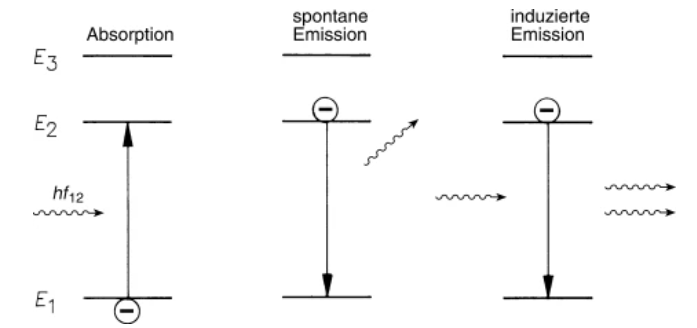
\includegraphics[scale=0.9]{pictures/Prozesse.png}
    \caption{Übergänge zwischen Energieniveaus\cite{Eichler20152}.}
    \label{fig:Prozesse}
\end{figure}
\noindent Damit die für den Laser wichtige Besetzungsinversion erzeugt wird, muss der Laser mindestens ein 3-Niveau-System besitzen.
Denn in einem 2-Niveau System würden sich stimulierte Emission und Absorption gegenseitig aufheben, da die Wahrscheinlichkeit für beide Prozesse gleich ist.
In einem Halbleiterlaser mit einer kontinuierlichen Bandstruktur ist dies automatisch gegeben.
\subsection{Halbleiter}
In Festkörpern mit einem periodischen Gitter kann die Besetzung der Elektronen über eine Bandstruktur beschrieben werden.
Nach dem Pauli-Prinzip können zwei Elektronen in einem System nicht die gleichen Energieniveaus besetzen. Daher spalten sich 
die Energieniveaus der einzelnen Atome in ein Band auf. Genauer sind die Energiebänder die Überlagerungen der Energieniveaus aller Atome im 
reziproken Raum. Dementsprechend können Elektronen mit einer bestimmten Energie im Festkörper nur vorliegen, wenn es Zustände in einem Band mit dieser 
Energie gibt. Energieintervalle ohne Zustand werden Bandlücken genannt, da dort keine Elektronen existieren können.

\noindent Festkörper können anhand ihrer Bandstruktur in 3 Kategorien unterteilt werden: Metalle, Halbleiter und Isolatoren.
Die Bandstruktur dieser Festkörper ist in Abbildung \ref{fig:Band} dargestellt.
\begin{figure}[H]
    \centering
    \includegraphics[scale=0.8]{pictures/Bänder.png}
    \caption{Bandstruktur von Metallen, Halbleitern und Isolatoren \cite{demtröder}.}
    \label{fig:Band}
\end{figure}
\noindent Dabei bezeichnet $E_\text{F}$ die Fermi-Energie, welche angibt bis zu welcher Energie bei $T=\qty{0}{\kelvin}$ die Zustände besetzt sind.
Bei Isolatoren liegt diese Energie zwischen 2 Bändern, also in einer Bandlücke. Das Band unterhalb der Fermi-Energie wird Valenzband genannt, 
da dieses bei $T=\qty{0}{\kelvin}$ vollständig besetzt ist. Das Band oberhalb der Fermi-Energie wird Leitungsband genannt, da dieses bei $T=\qty{0}{\kelvin}$ leer ist und 
Elektronen in diesem Band frei beweglich sind. Bei Metallen liegt die Fermi-Energie im Leitungsband, weshalb diese bei $T=\qty{0}{\kelvin}$ leitfähig sind.
Halbleiter haben eine analoge Bandstruktur zu Isolatoren, jedoch ist die Bandlücke kleiner. Sie beträgt bei Halbleitern bis zu $\qty{3}{\eV}$, bei Isolatoren 
ist sie größer. Daher können in Halbleitern durch thermische Anregung, bei Raumtemperatur etwa $\qty{26}{\milli\eV}$, Elektronen in das Leitungsband gelangen. 
Allerdings ist die Ladungsträgerdichte in Eigenleitung noch sehr gering. In diesem Versuch wird ein Aluminium-Gallium-Arsenid-Halbleiter (AlGaAs) verwendet. Dieser kann als "Light emitting Diode" (LED)
durch Rekombination von Elektronen und Löchern Licht emittieren. Die Bandlücke liegt im infrarotem Wellenlängenbereich von $\qty{780}{\nano\meter}$.
Entscheidend für die Funktionsweise eines Diodenlasers ist nun auch die Biegung der Bänder im p-n-Übergang. Bei angelegter Spannung können 
Driftströme das E-Feld der Verarmungszone überwinden und Ladungen sammeln sich bereit zum Rekombinieren in der Verarmungszone.
Dies ist schematisch in Abbildung \ref{fig:PN} dargestellt. 
\begin{figure}[H]
    \centering
    \includegraphics[scale=0.8]{pictures/PN-Übergang.png}
    \caption{Bänderdiagramm eines p-n-Übergangs \cite{Demtröder}.}
    \label{fig:PN}
\end{figure}
\subsection{Funktionsweise des Diodenlasers}
Der grundlegende Aufbau des verwendeten Halbleiterchips, der für diesen Laser verwendet wurde ist in Abbildung \ref{fig:Chip} dargestellt.
\begin{figure}[H]
    \centering
    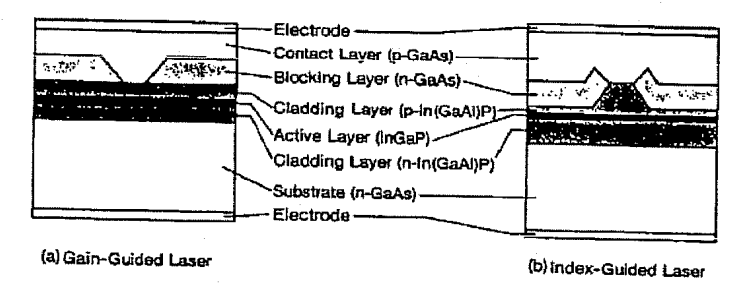
\includegraphics[scale=0.8]{pictures/Chip.png}
    \caption{Aufbau eines Halbleiterlasers \cite{teachspin}.}
    \label{fig:Chip}
\end{figure}
\noindent Grundlegend arbeitet der Laser wie eine LED, welche fortlaufend stimmuliert wird. Die Diode ist in Fließrichtung 
an eine äußere Spannung angeschlossen. Diese versorgt die Diode mit fortlaufend neuen Ladungen in der Sperrschicht 
zwischen p- und n-dotiertem Halbleiter müssen die Ladungen das innere elektrische Feld der Diode überwinden und sammeln sich deswegen in der Region des Übergangs.
Dies wird in Abbildung  \ref{fig:Chip} als aktive Schicht bezeichnet. Dort können Ladungen spontan mit Löchern unter Aussendung eines Photons rekombinieren.
Dies ist das Prinzip jeder LED. Dieses Licht ist allerdings weder allzu intensiv noch kohärent. Außerdem ist die Wellenlänge auf Grund der ausgedehnten Bänder 
noch nicht allzu präzise. Die Oberflächen des Kristalls sind nun so beschichtet, dass Sie sehr reflektierend sind. Dadurch passiert das Licht die aktive Schicht viele 
Male und induziert so durch stimmulierte Emission weitere Übergänge zwischen den Bändern. Das dabei entstehende Licht ist kohärent und bei genügend hohem Strom können sich 
innerhalb des Kristalls stehende Wellen mit festen Moden ausbilden. Dies wird innerer Resonator genannt.
Der Übergang zwischen den Bändern ist stark temperaturabhängig, weswegen die Wellenlänge mit dem höchsten Nettogewinn auch von der Temperatur abhängig ist.
Da durch den Halbleiter Strom fließt, kann auch durch die Stromstärke die Temperatur und somit die Wellenlänge eingestellt werden. 
Die Stromstärkenabhängigkeit ist in Abbildung \ref{fig:Strom} dargestellt.
\begin{figure}[H]
    \centering
    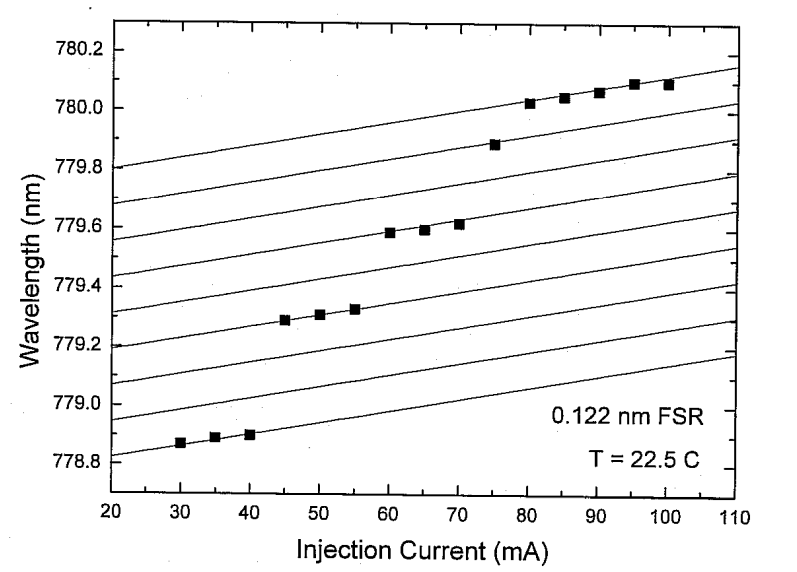
\includegraphics[scale=0.8]{pictures/Strom.png}
    \caption{Stromstärkenabhängigkeit der Wellenlänge eines Lasers \cite{teachspin}.}
    \label{fig:Strom}
\end{figure}

\subsection{Littrow-Konfiguration}
Die Littrow-Konfiguration ist eine spezielle Konfiguration eines Lasers, bei der ein Kristall als Resonatorspiegel dient.
Die Konfiguration ist in Abbildung \ref{fig:Littrow} dargestellt. Der reflektierte Anteil wird ausgekoppelt und kann für optische Experimente genutzt werden.
\begin{figure}[H]
    \centering
    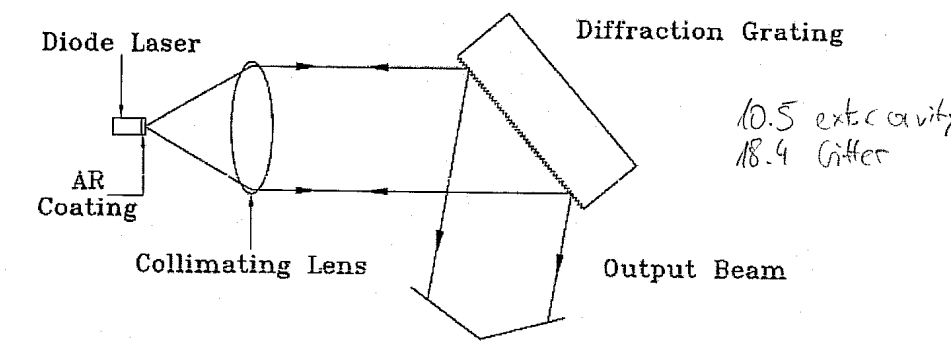
\includegraphics[scale=0.8]{pictures/Littrow.png}
    \caption{Littrow-Konfiguration eines Lasers \cite{teachspin}.}
    \label{fig:Littrow}
\end{figure}
\noindent Zusätzlich bilden sich jedoch gemäß der Bragg-Bedingung
\begin{equation}
    2d\sin(\theta)=m\lambda
\end{equation}
mit der Gitterkonstanten $d$, dem Beugungswinkel $\theta$, der Ordnung $m$ und der Wellenlänge $\lambda$ Beugungsmaxima aus. 
Der Kristall ist nun so positioniert, dass das 1. Beugungsmaximum auf den Halbleiter zurückfällt.
Der Anteil wird dann wieder im inneren Resonator verstärkt und irgendwann ausgekoppelt. Dadurch hat der Kristall 
die Wirkung eines weiteren Resonatorspiegels mit der Länge $L$. Damit bildet der Halbleiter mit dem Kristall einen externen Resonator
mit einer eigenen Modenstruktur. Auf Grund der größeren Länge liegen die einzelnen Moden gemäß 
\begin{equation}
    \Delta \nu = \frac{c}{2L}
\end{equation}
näher beieinander. Die Moden sind dafür schärfer. In Summe ergeben sich so 4 verschiedene Wellenlängenabhängigkeiten der Intensität.
Diese sind in Abbildung \ref{fig:Moden} dargestellt.
\begin{figure}[H]
    \centering
    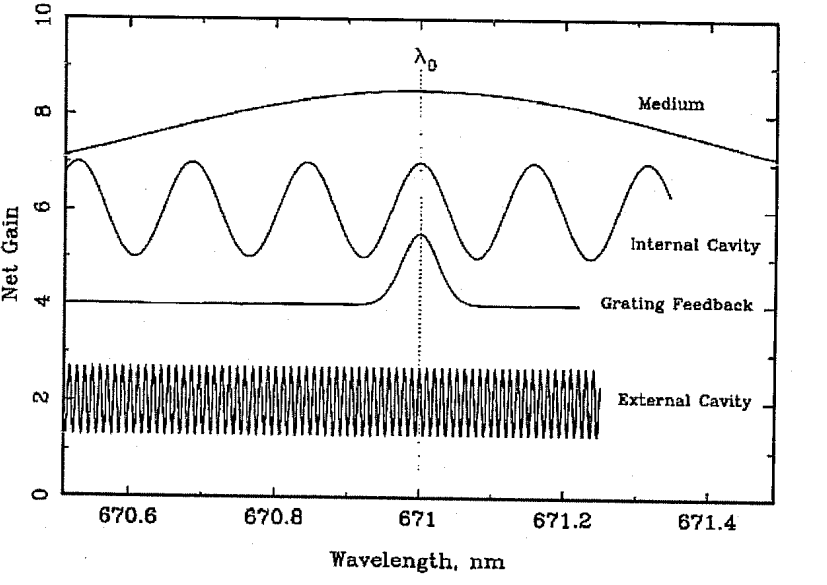
\includegraphics[scale=0.8]{pictures/Moden.png}
    \caption{Modenstruktur eines Lasers \cite{teachspin}.}
    \label{fig:Moden}
\end{figure}
\noindent Eine Überlagerung der Bragg-Bedingung mit dem externen Resonator führt zu der Intensitätsabhängigkeit in Abbildung \ref{fig:Moden1}.
\begin{figure}[H]
    \centering
    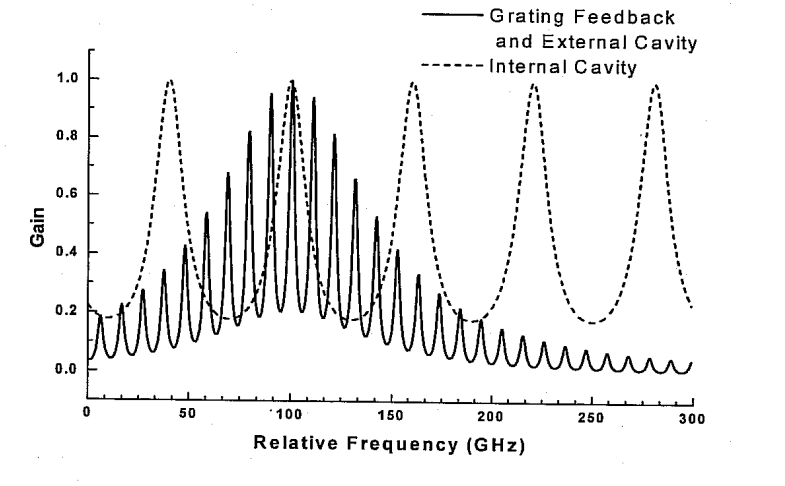
\includegraphics[scale=0.8]{pictures/Moden1.png}
    \caption{Intensitätsabhängigkeit der überlagerten Moden \cite{teachspin}.}
    \label{fig:Moden1}
\end{figure}
\noindent Nun kann über Veränderung des Kristallwinkels, des Stroms oder der Temperatur die Modenstruktur verschoben werden.
Da praktisch die gesamte Energie in einer Mode gespeichert wird, bildet sich immer nur die Mode mit dem höchsten Nettogewinn aus. 
Dies kann bei leichter Veränderung der Wellenlängenabhängigkeit, wie es beispielsweise in der Spektroskopie erwünscht ist, um einen schmalen 
Wellenlängenbereich zu untersuchen, zu "Mode Hopping"  führen wie es in Abbildung \ref{fig:Moden2} dargestellt ist.
\begin{figure}[H]
    \centering
    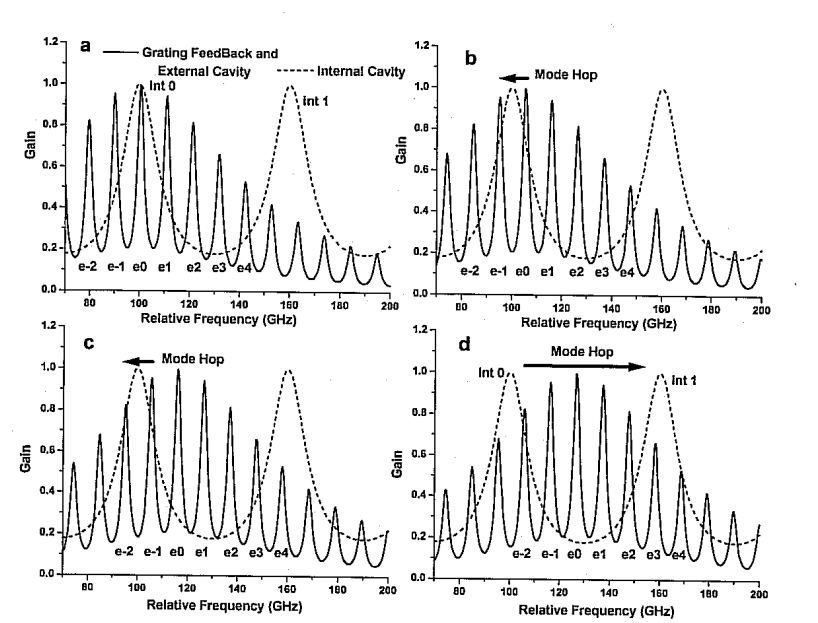
\includegraphics[scale=0.8]{pictures/Moden2.png}
    \caption{Mode Hoping eines Lasers \cite{teachspin}.}
    \label{fig:Moden2}
\end{figure}
\noindent Wenn sich die Maxima des externen Resonators zu sehr gegeneinander verschoben haben, wird ab einem bestimmten Punkt eine andere Interne Mode verstärkt und 
die Wellenlänge springt zwischen diesen beiden Inneren Moden. Für Spektroskopie sollte das vermieden werden.
\subsection{Hyperfeinstruktur des Rubidium-Spektrums}
Die nichtrelativistische Schrödingergleichung für das Wasserstoffatom liefert Energieniveaus, die allein von der Hauptquantenzahl \(n\) abhängen. Die Feinstruktur entsteht durch relativistische Spin-Bahn-Kopplung: 
Im Elektronenbezugssystem erzeugt die Bewegung des Kerns ein Magnetfeld, das mit dem Elektronenspin wechselwirkt und die Energieniveaus abhängig von der Spinrichtung differenziert.
Die Hyperfeinstruktur beruht auf der Wechselwirkung zwischen dem Kernspin \(I\) und dem Gesamtdrehimpuls \(J\) des Elektrons. Daraus ergibt sich der Gesamtdrehimpuls \(F\), der über die Beziehung 
\[
F = |I - J|, ..., I + J
\]
bestimmt wird. Für Elektronen im Grundzustand von Rubidium, welches als Alkalimetall Wasserstoff sehr ähnlich ist, (\(n=5\), \(L=0\), \(S=\frac{1}{2}\), \(J=\frac{1}{2}\)) gibt es bei einem Kernspin \(I=\frac{5}{2}\) die Werte \(F=2\) und \(F=3\)
und bei einem Kernspin \(I=\frac{3}{2}\) die Werte \(F=1\) und \(F=2\). Ein Termschema für den ersten Fall ist in Abbildung \ref{fig:Feinstruktur} dargestellt.
\begin{figure}
    \centering
    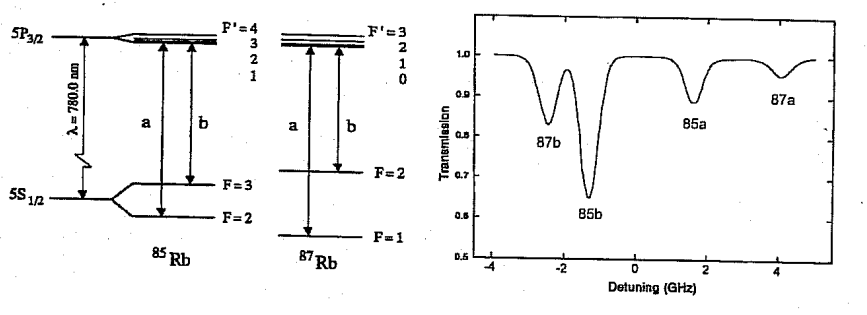
\includegraphics[width=\textwidth]{pictures/Term.png}
    \caption{Schematische Darstellung der Feinstruktur- und Hyperfeinstrukturaufspaltung}
    \label{fig:Feinstruktur}
\end{figure}
Im Rubidiumgas liegen nun 2 verschiedene Isotope vor, \(^{85}Rb\) und \(^{87}Rb\), die sich in ihrem Kernspin unterscheiden. Es gibt nun wie in 
Abbildung \ref{fig:Feinstruktur} dargestellt 2 verschiedene Übergänge für jedes Isotop mit leicht verschobenen Wellenlängen. Es sollten also 4 Peaks, 2 Hohe und 2 niedrige, vorkommen.
Die beiden hohen werden von \(^{85}Rb\) erzeugt, da diese Isotop mit 72\% gegenüber \(^{87}Rb\) häufiger vorkommt. 
%\cite{}
